\documentclass[11pt]{beamer}
\usepackage{amsfonts,amsmath,amsthm,amssymb}
\theoremstyle{plain}
\newtheorem{conjecture}{Conjecture}[section]
\usepackage{mathtools,mathptmx,listings,forest,enumitem}
\usepackage{graphicx}
\usepackage{pgfplots}
\pgfplotsset{compat=newest}
% plotting things
\usepackage{graphicx}
\graphicspath{{images/}}
\usepackage{tikz-cd}
\pgfplotsset{compat=1.15}
\usepackage[
	backend=biber,
	style=verbose,
	sorting=ynt
]{biblatex}
\addbibresource{references.bib}
\usetheme{Madrid}
\usepackage{float,mathtools,dirtytalk,ulem,csquotes,cancel,hyperref}
\author[] % (optional)
{Emon Hossain\inst{1}}

\institute[University of Dhaka] % (optional)
{
  \inst{1}%
  Lecturer\\
  emon.hossain@bracu.ac.bd\\
  \\MNS department\\Brac University
}

\date[] % (optional)
{\textsc{Lecture-01}}


\title[]{MAT216: Linear Algebra and Fourier Transformation}

\setbeamertemplate{navigation symbols}{}


\AtBeginSection[]
{
  \begin{frame}
    \frametitle{Table of Contents}
    \tableofcontents[currentsection]
  \end{frame}
}

\usepackage{Kyushu}

% \usetheme{Frankfurt}

\begin{document}

\begin{frame}
\titlepage
\end{frame}

\section{Motivation}
\begin{frame}{simple system}
System of equations is the most fascinating topic in Linear Algebra. Because we can see it through both vector space and Linear Transformation perspective respectively. For example, take a system of linear equations,
\begin{align}
\begin{split}
    x-y&=1\\
    2x+y&=6
\end{split}
\end{align}
\pause
\begin{align*}
    \begin{pmatrix}
        1\\2
    \end{pmatrix}x+\begin{pmatrix}
        -1\\1
    \end{pmatrix}y=\begin{pmatrix}
        1\\6
    \end{pmatrix}
\end{align*}
\pause
\textbf{Interpretation of the solution:} Here, we want to find such scalars $x,y$ for which our vectors $\begin{pmatrix}
    1\\2
\end{pmatrix}$ and $\begin{pmatrix}
    -1\\1
\end{pmatrix}$ can reach the vector $\begin{pmatrix}
    1\\6
\end{pmatrix}$ by \textbf{vector addition}.
%     \begin{displayquote}
% \end{displayquote}
\end{frame}

\begin{frame}{Matrix form}
Likewise, we can rewrite the system as,
\begin{align*}
    \begin{pmatrix}
        1 & -1\\
        2 & 1
    \end{pmatrix}\begin{pmatrix}
        x\\y
    \end{pmatrix}=\begin{pmatrix}
        1\\6
    \end{pmatrix}
\end{align*}
Here, we are considering the linear transformation (don't worry we will discuss it in our upcoming lectures, or if you want to understand it right now have a look at the course \href{https://www.youtube.com/watch?v=fNk_zzaMoSs&list=PLZHQObOWTQDPD3MizzM2xVFitgF8hE_ab}{Essence of linear algebra}, YouTube playlist from 3b1b channel) and want to find such vectors which are mapped to the specific vector $\begin{pmatrix}
    1\\6
\end{pmatrix}$ after the transformation applied.\\
\pause
\textbf{Interpretation of the solution:} So, basically we want all those vectors $\begin{pmatrix}
    x\\y
\end{pmatrix}$ which are mapped to $\begin{pmatrix}
    1\\6
\end{pmatrix}$.
\end{frame}

\begin{frame}{Bigger picture}
\begin{center}
	\begin{forest}
		for tree={%
			align=center, %% ADDED
			edge path={\noexpand\path[\forestoption{edge}] (\forestOve{\forestove{@parent}}{name}.parent anchor) -- +(0,-12pt)-| (\forestove{name}.child anchor)\forestoption{edge label};}
		}
		[
		System of linear Equations,
		[Algebraic form]
		[Vector form]
		[Transformation form]
        [$\cdots$]
		]
	\end{forest}
\end{center}
\pause
\begin{figure}[H]
\centering

\includegraphics[scale=0.3]{madness.jpeg}
\end{figure}
Welcome to Linear Algebra, where the notation is made up and you might gain your third eye.
\begin{displayquote}
\say{Life isn't linear, but written words are. Like our system of linear equations.}
\end{displayquote}
\end{frame}

\begin{frame}{System of equation: Two variables}
\begin{figure}[H]
\centering
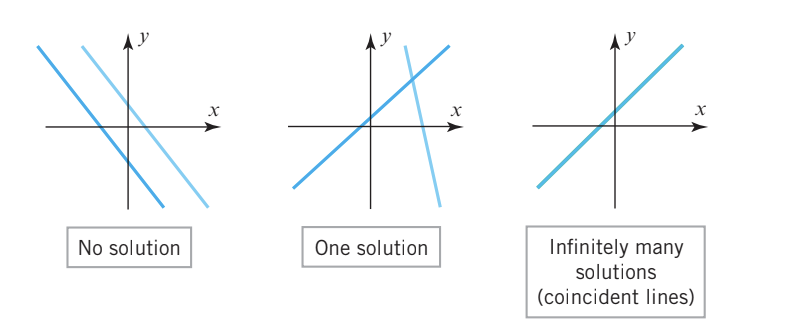
\includegraphics[scale=0.5]{L1 lines.png}
\end{figure}
\end{frame}

\begin{frame}{System of equation: Three variables}
\begin{figure}[H]
\centering
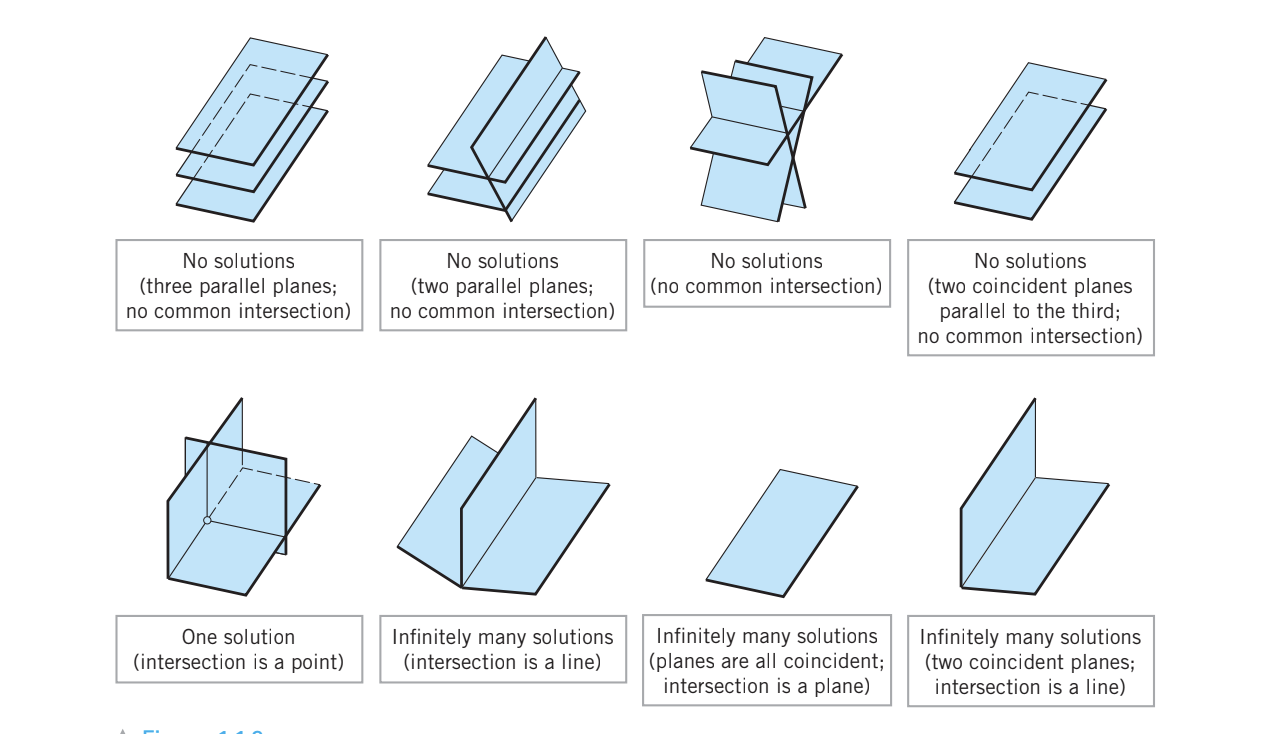
\includegraphics[scale=0.5]{L1 planes.png}
\end{figure}
\end{frame}

\begin{frame}{continued...}
Like for a three-variable system:
$$
\begin{cases}
    a_1x+b_1y+c_1z&=d_1\\
    a_2x+b_2y+c_2z&=d_2\\
    a_3x+b_3y+c_3z&=d_3
\end{cases}
$$
We can rewrite it in the vector form:
$$
\underbrace{\begin{pmatrix}
    a_1\\a_2\\a_3
\end{pmatrix}}_{\in\mathbb R_3}x+
\underbrace{\begin{pmatrix}
    b_1\\b_2\\b_3
\end{pmatrix}}_{\in\mathbb R_3}y+
\underbrace{\begin{pmatrix}
    c_1\\c_2\\c_3
\end{pmatrix}}_{\in\mathbb R_3}z=
\underbrace{\begin{pmatrix}
    d_1\\d_2\\d_3
\end{pmatrix}}_{\in\mathbb R_3}
$$
\end{frame}
\begin{frame}{continued...}
So, our solution $\begin{pmatrix}
    x\\y\\z
\end{pmatrix}$ actually tell us how much we should scale our column vectors $\begin{pmatrix}
    a_1\\a_2\\a_3
\end{pmatrix},\begin{pmatrix}
    b_1\\b_2\\b_3
\end{pmatrix}$ and $\begin{pmatrix}
    c_1\\c_2\\c_3
\end{pmatrix}$ respectively in order to reach the right hand side vector $\begin{pmatrix}
    d_1\\d_2\\d_3
\end{pmatrix}$.\\
Two questions that we will revisit many times throughout our course: (1) Does a given linear system have a solution? In other words, is it consistent? (2) If it is consistent, is the solution unique?
\end{frame}
\begin{frame}{Course outline}
\begin{figure}[H]
\centering
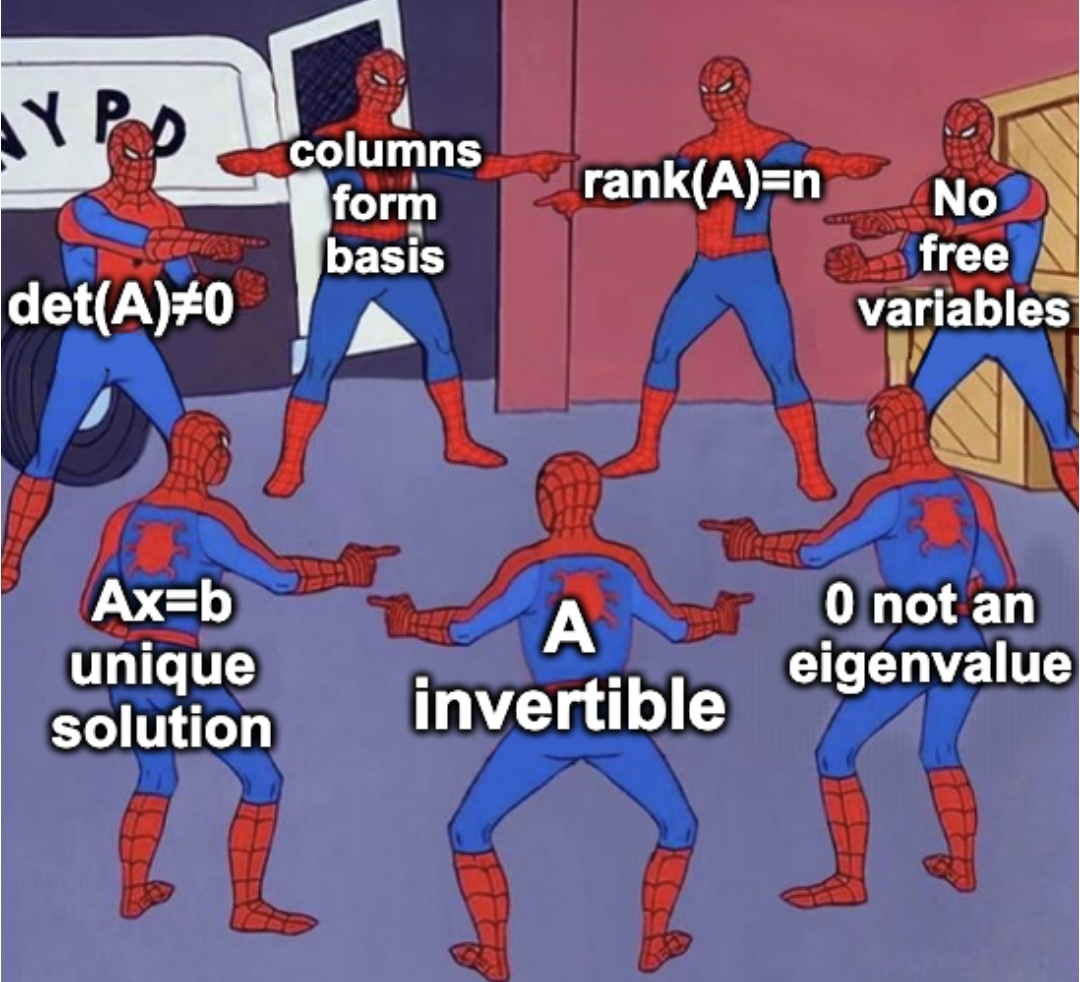
\includegraphics[scale=0.2]{outline.png}
\end{figure}
\end{frame}
\begin{frame}{Questions}
    .
\end{frame}
\begin{frame}{continued...}
    .
\end{frame}

\section{Bibliography}
\begin{frame}[t,allowframebreaks]
\frametitle{Bibliography}
\printbibliography[heading=none]
\end{frame}
\end{document}
